%%%%%%%%%%%%%%%%%%%%%%%%%%%%%%%%%%%%%%%%%%%%%%%%%%%%%%%%%%%%%%%%%%%%%%%%%%%%%%%
%                       CARREGA DE LA CLASSE DE DOCUMENT                      %
%                                                                             %
% Les opcions admissibles son:                                                %
%      12pt / 11pt            (cos dels tipus de lletra; no feu servir 10pt)  %
%                                                                             %
% catalan/spanish/english     (llengua principal del treball)                 %
%                                                                             % 
% french/italian/german...    (si necessiteu fer servir alguna altra llengua) %
%                                                                             %
% listoffigures               (El document inclou un Index de figures)        %
% listoftables                (El document inclou un Index de taules)         %
% listofquadres               (El document inclou un Index de quadres)        %
% listofalgorithms            (El document inclou un Index d'algorismes)      %
%                                                                             %
%%%%%%%%%%%%%%%%%%%%%%%%%%%%%%%%%%%%%%%%%%%%%%%%%%%%%%%%%%%%%%%%%%%%%%%%%%%%%%%

\documentclass[11pt,spanish,listoffigures,listoftables]{tfgetsinf}

%%%%%%%%%%%%%%%%%%%%%%%%%%%%%%%%%%%%%%%%%%%%%%%%%%%%%%%%%%%%%%%%%%%%%%%%%%%%%%%
%                     CODIFICACIO DEL FITXER FONT                             %
%                                                                             %
%    windows fa servir normalment 'ansinew'                                   %
%    amb linux es possible que siga 'latin1' o 'latin9'                       %
%    Pero el mes recomanable es fer servir utf8 (unicode 8)                   %
%                                          (si el vostre editor ho permet)    % 
%%%%%%%%%%%%%%%%%%%%%%%%%%%%%%%%%%%%%%%%%%%%%%%%%%%%%%%%%%%%%%%%%%%%%%%%%%%%%%%

\usepackage[utf8]{inputenc} 

%%%%%%%%%%%%%%%%%%%%%%%%%%%%%%%%%%%%%%%%%%%%%%%%%%%%%%%%%%%%%%%%%%%%%%%%%%%%%%%
%                        ALTRES PAQUETS I DEFINICIONS                         %
%                                                                             %
% Carregueu aci els paquets que necessiteu i declareu les comandes i entorns  %
%                                          (aquesta seccio pot ser buida)     %
%%%%%%%%%%%%%%%%%%%%%%%%%%%%%%%%%%%%%%%%%%%%%%%%%%%%%%%%%%%%%%%%%%%%%%%%%%%%%%%



%%%%%%%%%%%%%%%%%%%%%%%%%%%%%%%%%%%%%%%%%%%%%%%%%%%%%%%%%%%%%%%%%%%%%%%%%%%%%%%
%                        DADES DEL TREBALL                                    %
%                                                                             %
% titol, alumne, tutor i curs academic                                        %
%%%%%%%%%%%%%%%%%%%%%%%%%%%%%%%%%%%%%%%%%%%%%%%%%%%%%%%%%%%%%%%%%%%%%%%%%%%%%%%

\title{Implementación de sensores geolocalizados para la obtención de datos en un área metropolitana}
\author{\textbf{David Rodriguez Martinez}}
\tutor{\textbf{David Cuesta Frau}}
\curs{\textbf{2015-2016}}

%%%%%%%%%%%%%%%%%%%%%%%%%%%%%%%%%%%%%%%%%%%%%%%%%%%%%%%%%%%%%%%%%%%%%%%%%%%%%%%
%                     PARAULES CLAU/PALABRAS CLAVE/KEY WORDS                  %
%                                                                             %
% Independentment de la llengua del treball, s'hi han d'incloure              %
% les paraules clau i el resum en els tres idiomes                            %
%%%%%%%%%%%%%%%%%%%%%%%%%%%%%%%%%%%%%%%%%%%%%%%%%%%%%%%%%%%%%%%%%%%%%%%%%%%%%%%

\keywords{Ciutat Inteligent, Arduino, Hardware, Geolocalizació, Sensors, Harware lliure, Electrònica, Servicis Web} % Paraules clau 
         {Ciudad Inteligente, Arduino, Hardware, Geolocalizacion, Sensores, Harware Libre, Electronica, Servicios Web}              % Palabras clave
         {Arduino, Smart City, IoT, Remote Sensor, Open-source hardware}        % Key words
         
         %Arduino, Hardware Libre, Sensores, Control Remoto, Servidor Web, Electrónica, Arduino Shield, GPS.

%%%%%%%%%%%%%%%%%%%%%%%%%%%%%%%%%%%%%%%%%%%%%%%%%%%%%%%%%%%%%%%%%%%%%%%%%%%%%%%
%                              INICI DEL DOCUMENT                             %
%%%%%%%%%%%%%%%%%%%%%%%%%%%%%%%%%%%%%%%%%%%%%%%%%%%%%%%%%%%%%%%%%%%%%%%%%%%%%%%

\begin{document}

%%%%%%%%%%%%%%%%%%%%%%%%%%%%%%%%%%%%%%%%%%%%%%%%%%%%%%%%%%%%%%%%%%%%%%%%%%%%%%%
%              RESUMS DEL TFG EN VALENCIA, CASTELLA I ANGLES                  %
%%%%%%%%%%%%%%%%%%%%%%%%%%%%%%%%%%%%%%%%%%%%%%%%%%%%%%%%%%%%%%%%%%%%%%%%%%%%%%%


\begin{abstract}[spanish]
	
	El motivo de este proyecto es utilizar una plataforma de “hardware libre” llamada Arduino con el fin de implementar uno o varios nodos de sensores el cual enviará a través de la red Información sobre un área específica, y podremos monitorizar la informacion gracias a una aplicacion web.
	
	Mi intención es que gracias a lo explicado en el párrafo anterior se pueda implementar una utilidad hardware y una Web para utilizar en una Smart City\\
	
	\end{abstract}
\begin{abstract}

	El motiu d'aquest projecte es utilitzar una plataforma de "hardware lliure" anomenada arduino amb l'intencio d'implementar u o varios nodes de sensors, el cual enviara utilitzant una xarxa, informacio sobre una área específica la cual podrem monitoritzar gracies a una aplicació web . 

	La meua intenció es que gracies a el que he explicat en el parraf anterior es puga implementar una utilitat de gestió per utilitzar en una Smart City\\


\end{abstract}
\begin{abstract}[english]
	The purpose of this project is use a special Open-source hardware platform called Arduino, with the intention of implement one or more nodes of sensors, which will send on the network, information about a specific area that we can monitoring, using a web service.
	
	My intention is that thanks to I've explained in the last paragraph, i will can implement a hardware and web application to track that information to use in the future in the Smart city.\\

	
\end{abstract}

%%%%%%%%%%%%%%%%%%%%%%%%%%%%%%%%%%%%%%%%%%%%%%%%%%%%%%%%%%%%%%%%%%%%%%%%%%%%%%%
%                              CONTINGUT DEL TREBALL                          %
%%%%%%%%%%%%%%%%%%%%%%%%%%%%%%%%%%%%%%%%%%%%%%%%%%%%%%%%%%%%%%%%%%%%%%%%%%%%%%%

\mainmatter

%%%%%%%%%%%%%%%%%%%%%%%%%%%%%%%%%%%%%%%%%%%%%%%%%%%%%%%%%%%%%%%%%%%%%%%%%%%%%%%
%                                  INTRODUCCIO                                %
%%%%%%%%%%%%%%%%%%%%%%%%%%%%%%%%%%%%%%%%%%%%%%%%%%%%%%%%%%%%%%%%%%%%%%%%%%%%%%%


\chapter{Introducción a la práctica}

Esta práctica de Lenguajes y entornos de programación paralela consiste en la explotación de la GPU con el fin de poder obtener unos resultados de ejecución de problemas pesados para poder ser comparados entre diversos dispositivos y modelos de ejecución a fin de saber cuánta mejora ofrece este sistema de procesamiento.

El cálculo acelerado es el uso de una unidad de procesamiento gráfico en combinación con una CPU para acelerar aplicaciones de empresa, ingeniería, análisis y cálculo científico.\\
Gracias a esto las GPU aceleradoras han pasado a instalarse en centros de datos energéticamente eficientes de laboratorios gubernamentales, universidades y grandes compañías de todo el mundo. Las GPUs aceleran las aplicaciones de plataformas diversas, desde automóviles hasta teléfonos móviles y tablets, drones y robots.

Para ello he realizado la práctica bajo \textit{OpenCL}, una serie de librerías aportadas por \textit{CUDA GPU Programming}.

Con esto implementaremos un código en C que incorpora este modelo de programacion paralela que se ejecutara numerosas veces mientras se le aumenta la talla del problema, además se compararán diversas tecnologías, como la explotación de un solo núcleo (programación secuencial), \textit{CUDA} y \textit{OpenCL} (programación paralela) a fin de obtener una serie de resultados en los que se aplicaran diferentes comparaciones y conclusiones.

Además OpenCL es una especificación desarrollada por Apple, asi que se realizara una prueba en un entorno que incorpora nativamente OpenCL (OS X) con el fin de ver cómo de sencillo resulta trabajar con esta especificación en un entorno preparado.


%\section{Notes bibliografiques} %%%%% Opcional

%????? ????????????? ????????????? ????????????? ????????????? ?????????????

%%%%%%%%%%%%%%%%%%%%%%%%%%%%%%%%%%%%%%%%%%%%%%%%%%%%%%%%%%%%%%%%%%%%%%%%%%%%%%%
%                         CAPITOLS (tants com calga)                          %
%%%%%%%%%%%%%%%%%%%%%%%%%%%%%%%%%%%%%%%%%%%%%%%%%%%%%%%%%%%%%%%%%%%%%%%%%%%%%%%

\chapter{Estudio del Arte}

\setlength{\parindent}{5ex}En este capitulo se hablara de porque se han elegido las tecnologías que se van a utilizar en el proyecto asi como mostrar algunas de las opciones adicionales que se podrían haber utilizado. 

\section{¿Porque Arduino?}

Arduino es una plataforma Hardware Open Source lo que implica que todo el sistema esta disponible a los usuarios y esto ayudara al proceso de montaje ya que una gran parte de personas (la comunidad de Arduino) trabajan de manera desinteresada en el desarrollo de librerías y aplicaciones para esta plataforma. 
\setlength{\parindent}{0ex}

Sin embargo Arduino dispone de numerosas versiones por lo que dentro de las mas famosas que hay he decidido analizar cual de los que hay me ofrece mas garantías a la hora de realizar el proyecto por lo que en principio me decantare por el consumo de las microcontroladora, puertos y conexiones disponibles y disponibilidad.

En primer lugar he realizado un estudio del consumo de las placas disponibles para poder realizar este proyecto, 

\begin{center}
	\begin{tabular}{c c c } 
		\hline
		\textbf{Board} & \textbf{Consumo(W/h)} & \textbf{Consumo(mA/h)} \\ [0.3ex] 
		\specialrule{.08em}{1em}{0em}
		Arduino UNO & 0.23 & 46  \\ 
		Arduino DUE & 0.375 & 75  \\
		Arduino MEGA & 0.465 & 93  \\
		Arduino Nano & 0.075 & 15  \\
		Raspberry Pi & 1.77 & 353  \\ [1ex] 
		\hline
	\end{tabular}
	\captionof{table}{Consumo de los diferentes dispositivos} \label{tab:table1} 
\end{center}

En este caso nos interesaría el elegir el dispositivo que menor consumo tenga pero también he tenido que mirar que funcionalidad pueden aportar cada placa, cabe destacar que la Raspberry Pi no es una microcontroladora, si no un ordenador de placa reducida, pero ofrece una funcionalidad que podría mejorar las prestaciones de este proyecto, hablando de seguridad y comunicación, pero sin embargo después de las pruebas de consumo comparando con el Arduino que mas consume, en este caso el MEGA, consume en mA un 379\% mas ya que necesita mantener un sistema operativo que aunque sigue siendo un consumo muy bajo para ser un ordenador, es muy elevado para este proyecto así que en este punto descartamos la Raspberry Pi.

Otro punto a tener en cuenta son las capacidades de conexión que tienen las microcontroladoras, ya que para poder conectarlo todo voy a necesitar 3 entradas analógicas, una  entrada digital, 2 entradas para el rx y tx del puerto serie y compatibilidad con la Shield ethernet de Arduino.

El Arduino UNO es una muy buena opción ya que tiene todo esto y es de un consumo reducido aun así, la comunicación serial va por software ya que hay que implementar una librería especial para poder realzar un puerto serie para comunicarse con el GPS, ademas habría que diseñar un circuito por los problemas en los voltajes de las lecturas digitales ya que algunos componentes devuelven 3.3V y Arduino los detecta a 5V, que bien que no daría problemas pero podría dar lugar a valores anómalos en determinadas ocasiones.

El Arduino MEGA es la mejor opción disponible sin embargo ajustando con el material disponible, he de elegir el Arduino DUE ya que tiene un consumo mas reducido.

Estas son las características del Arduino DUE:

\begin{itemize}
\item \textbf{Microcontrolador}: AT91SAM3X8E
\item \textbf{Velocidad de reloj:} 84 MHz
\item \underline{\textbf{Tensión de trabajo:} 3.3V}
\item \underline{\textbf{Pines de entradas digitales:} 54}
\item \underline{\textbf{Pines de entradas analógicas: }12}
\item \underline{\textbf{Memoria Flash:} 512 KB}
\end{itemize}

He subrayado los valores que son importantes ya que en el estudio del montaje en el Arduino UNO tenia problemas con la memoria del programa ya que la memoria Flash quedaba casi completa utilizando la librería que implementaba un serial en cualquier pin digital,  imposibilitando la capacidad de poder implementar mejoras en la aplicación.

\section{Presupuesto}

En esta parte del proyecto se va a realizar un estudio de lo que puede llegar a costar la creación, el montaje y el mantenimiento de la aplicación, todo ello al precio actual del año 2016.

Em primer lugar se expondrá el coste de que costaría aproximadamente cada nodo de la aplicación:

\begin{itemize}
	\item \textbf{Arduino DUE:} 36\euro 
	\item \textbf{Shield de Ethernet:} 26\euro 
	\item \textbf{Neo6Mv2:} 13,50\euro 
	\item \textbf{Sensor de Gas MQ-7:} 8\euro 
	\item \textbf{Sensor de Temperatura y Humedad DHT11:} 3\euro 
	\item \textbf{Sensor de Sonido:} 0,50\euro 
	\item \textbf{Sensor de Luz:} 1\euro 
\end{itemize}

Todo esto nos da un coste de \textbf{88 \euro} por nodo de sensores aproximadamente.

Se podrían utilizar materiales mas baratos con el fin de reducir los costes aun mas pero no seria aconsejable pues del proyecto interesa que este activo el mayor tiempo posible. También se pueden modificar los elementos del mismo, nombrados en la parte donde se realizaba el estudio del consumo de energía de cada controladora (\textbf{Tabla \ref{tab:table1}}) realizando las modificaciones necesarias para que este pueda funcionar.

También se ha incluido el coste de lo que costaría añadir el servidor de la aplicación, en este caso he puesto componentes genéricos:

\begin{itemize}
	\item \textbf{Servidor:} 600\euro 
	\item \textbf{Router:} 30\euro 
	\item \textbf{Cableado:} 12\euro 
\end{itemize}

Todo esto nos da un coste de \textbf{642 \euro} por servidor aproximadamente, pero, como se ha explicado antes, todo esto se puede reducir con material ya disponible, porque, "quien no tiene un ordenador hoy día?".

Y por ultimo el mantenimiento de lo que seria todo el montaje, ya es difícil hablar de un mantenimiento pues la aplicación pues aumentaría con cada nodo añadido, la ampliación del servidor en caso de haber demasiadas peticiones, el modo de alimentar los nodos que podría ser por microUSB, POE o baterías, diferentes Controladoras, todo esto nos daría un resultado muy variable, así que es muy complicado cuanto costaría mantener la aplicación.

\section{Gestión del proyecto}

Para este proyecto se va a gestionar el proyecto utilizando una aplicación Web llamada \textit{Bitbucket}:

\textit{Bitbucket es un servicio de alojamiento basado en web, para los proyectos que utilizan el sistema de control de revisiones Mercurial y Git.}\cite{bitbucket}.

En esta aplicación se irán subiendo todos los cambios que se realicen en este proyecto ya que ofrece una gestión bastante sencilla de los proyectos y las versiones de cada una, ademas cuenta con una aplicación llamada \textit{sourceTree} que permite conectar con una cuenta de \textit{Bitbucket} y permitirá realizar las subidas de ficheros desde el mismo sistema operativo sin tener que acceder desde el navegador y ademas gestionar de una manera sencilla todas las versiones del proyecto.

\begin{figure}[!h]
	\centering
	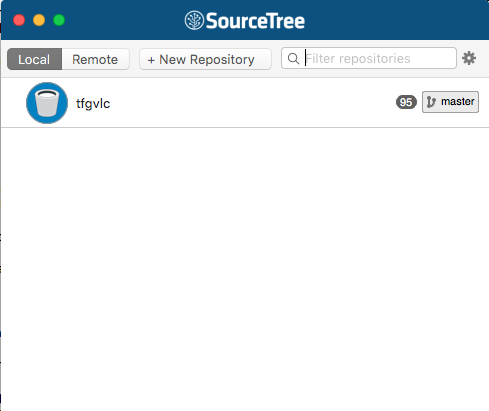
\includegraphics[width=0.3\linewidth]{figuras/stree}
	\caption{Gestion de proyectos con \textit{SourceTree}}
	\label{fig:stree}
\end{figure}


\chapter{??? ???? ??????}

????? ????????????? ????????????? ????????????? ????????????? ?????????????

\section{?? ???? ???? ? ?? ??}

????? ????????????? ????????????? ????????????? ????????????? ?????????????

\chapter{??? ???? ??????}

????? ????????????? ????????????? ????????????? ????????????? ????????????? 

\section{?? ???? ???? ? ?? ??}

????? ????????????? ????????????? ????????????? ????????????? ?????????????

%%%%%%%%%%%%%%%%%%%%%%%%%%%%%%%%%%%%%%%%%%%%%%%%%%%%%%%%%%%%%%%%%%%%%%%%%%%%%%%
%                                 CONCLUSIONS                                 %
%%%%%%%%%%%%%%%%%%%%%%%%%%%%%%%%%%%%%%%%%%%%%%%%%%%%%%%%%%%%%%%%%%%%%%%%%%%%%%%

\chapter{Conclusiones}

????? ????????????? ????????????? ????????????? ????????????? ????????????? 

%%%%%%%%%%%%%%%%%%%%%%%%%%%%%%%%%%%%%%%%%%%%%%%%%%%%%%%%%%%%%%%%%%%%%%%%%%%%%%%
%                                BIBLIOGRAFIA                                 %
%%%%%%%%%%%%%%%%%%%%%%%%%%%%%%%%%%%%%%%%%%%%%%%%%%%%%%%%%%%%%%%%%%%%%%%%%%%%%%%

\begin{thebibliography}{10}

%%%%%%%%%%%%%%%%%%%%%%%%%%%%%%%%%%%%%%%%%%%%%%%%%%%%%%%%%%%%%%%%%%%%%%%%%%%%%%%
% MODEL D'ARTICLE                                                             %
%%%%%%%%%%%%%%%%%%%%%%%%%%%%%%%%%%%%%%%%%%%%%%%%%%%%%%%%%%%%%%%%%%%%%%%%%%%%%%%
%\bibitem{light}
%Jennifer~S. Light.
%\newblock When computers were women.
%\newblock \textit{Technology and Culture}, 40:3:455--483, juliol, 1999.

%%%%%%%%%%%%%%%%%%%%%%%%%%%%%%%%%%%%%%%%%%%%%%%%%%%%%%%%%%%%%%%%%%%%%%%%%%%%%%%
% MODEL DE LLIBRE                                                             %
%%%%%%%%%%%%%%%%%%%%%%%%%%%%%%%%%%%%%%%%%%%%%%%%%%%%%%%%%%%%%%%%%%%%%%%%%%%%%%%
%\bibitem{ifrah}
%Georges Ifrah.
%\newblock \textit{Historia universal de las cifras}.
%\newblock Espasa Calpe, S.A., Madrid, sisena edició, 2008.

%%%%%%%%%%%%%%%%%%%%%%%%%%%%%%%%%%%%%%%%%%%%%%%%%%%%%%%%%%%%%%%%%%%%%%%%%%%%%%%
% MODEL D'URL                                                                 %
%%%%%%%%%%%%%%%%%%%%%%%%%%%%%%%%%%%%%%%%%%%%%%%%%%%%%%%%%%%%%%%%%%%%%%%%%%%%%%%
\bibitem{Arduino}
Información sobre la redacción del TFG
\newblock consultado en 
\url{https://riunet.upv.es/}.

\bibitem{Arduino}
Información sobre Arduino DUE, conexiones y funcionamiento
\newblock consultado en 
\url{https://www.arduino.cc/en/Main/ArduinoBoardDue}.

\bibitem{NEO6mv2}
Información, decodificación, programación y DataSheet del dispositivo de Localización NEO6mv2 utilizado en el proyecto
\newblock consultado en \\
\url{https://www.u-blox.com/sites/default/files/products/documents/NEO-6_DataSheet_(GPS.G6-HW-09005).pdf}.\\
\url{http://www.gpsinformation.org/dale/nmea.htm}.\\
\url{http://arduiniana.org/libraries/tinygps/}

\bibitem{DHT11}
Información del funcionamiento y librerías del sensor DHT11
\newblock consultado en 
\url{http://playground.arduino.cc/Main/DHT11Lib}.\\
\url{https://cdn-learn.adafruit.com/downloads/pdf/dht.pdf}.

\bibitem{Parallax Gas CO sensor}
Información del funcionamiento y DataSheet del sensor Parallax Gas CO sensor MQ-7
\newblock consultado en 
\url{https://www.parallax.com/sites/default/files/downloads/27904-Gas-Sensor-Modules-Guide-v2.3.pdf}.

\bibitem{Laravel 5.2}
Información sobre como desarrollar una aplicación WEB utilizando el Framework Laravel 5.2
\newblock consultado en 
\url{https://laravel.com/docs/5.2}.


\end{thebibliography}
\cleardoublepage

%%%%%%%%%%%%%%%%%%%%%%%%%%%%%%%%%%%%%%%%%%%%%%%%%%%%%%%%%%%%%%%%%%%%%%%%%%%%%%%
%                           APÈNDIXS  (Si n'hi ha!)                           %
%%%%%%%%%%%%%%%%%%%%%%%%%%%%%%%%%%%%%%%%%%%%%%%%%%%%%%%%%%%%%%%%%%%%%%%%%%%%%%%

\APPENDIX

%%%%%%%%%%%%%%%%%%%%%%%%%%%%%%%%%%%%%%%%%%%%%%%%%%%%%%%%%%%%%%%%%%%%%%%%%%%%%%%
%                         LA CONFIGURACIO DEL SISTEMA                         %
%%%%%%%%%%%%%%%%%%%%%%%%%%%%%%%%%%%%%%%%%%%%%%%%%%%%%%%%%%%%%%%%%%%%%%%%%%%%%%%

\chapter{Configuración del sistema}

????? ????????????? ????????????? ????????????? ????????????? ?????????????

\section{Fase d'inicialització}

????? ????????????? ????????????? ????????????? ????????????? ?????????????

\section{Identificació de dispositius}

????? ????????????? ????????????? ????????????? ????????????? ?????????????

%%%%%%%%%%%%%%%%%%%%%%%%%%%%%%%%%%%%%%%%%%%%%%%%%%%%%%%%%%%%%%%%%%%%%%%%%%%%%%%
%                               ALTRES  APÈNDIXS                              %
%%%%%%%%%%%%%%%%%%%%%%%%%%%%%%%%%%%%%%%%%%%%%%%%%%%%%%%%%%%%%%%%%%%%%%%%%%%%%%%


\chapter{??? ???????????? ????}

????? ????????????? ????????????? ????????????? ????????????? ????????????? 



%%%%%%%%%%%%%%%%%%%%%%%%%%%%%%%%%%%%%%%%%%%%%%%%%%%%%%%%%%%%%%%%%%%%%%%%%%%%%%%
%                              FI DEL DOCUMENT                                %
%%%%%%%%%%%%%%%%%%%%%%%%%%%%%%%%%%%%%%%%%%%%%%%%%%%%%%%%%%%%%%%%%%%%%%%%%%%%%%%

\end{document}
